%************************************************
\chapter{Curating a set of genome-wide orthologous mammalian gene alignments}
\label{ch_orthologs}
%************************************************

\section{Introduction}

The first step in any evolutionary sequence analysis is the collection
of homologous sequence data \citep{TODO}. 

\draft{The evolutionary history of vertebrate and mammalian genomes is
  diverse, full of genome duplications, and well-characterized relative to other species groups}

\draft{Still, availability of orthologous coding alignments is limited, and orthology itself is often uncertain}

\tocite{Jun2009}{They give good reasons for why orthology inference is still difficult}

\tocite{Ruan2008}{Provides a non-Compara example of tree-based
  orthology pipelines, and show that their 17k gene trees only cover
  ~84.5\% of genes}

\draft{Genomic alignments would seem to be ideal for use as an input
  source, except for the important issues of genome / segmental
  duplications}

\draft{As preparation for the mammalian analysis presented in chapters
  3 and 4, I undertook a small project to identify the best set of
  orthologs to use in an analysis of mammalian protein-coding
  genes. Part of the goal was to understand what taxonomic constraints
  best identify largely-orthologous groups of mammalian genes, and
  part was to evaluate whether low-coverage genomes showed high enough
  annotation quality to be included in the analysis.}

\section{Low-coverage genomes in the Ensembl database}

The prevalence of missing sequence data and fragmented contigs in
low-coverage genomes presents a unique set of problems for the
generation of transcript annotations. In recognition of these
differences, the procedure used by the Ensembl database to annotate
genomes assembled from low-coverage data is distinct from the usual
gene-building pipeline \citep{Hubbard2007}. Briefly, a whole-genome
alignment is produced between the human genome and each low-coverage
target, and gene models are projected from human to the target
genome. Small frame-disrupting insertions or deletions within
orthologous exons are corrected, and missing exons are padded with Ns
in order to obtain the correct transcript length.

The inclusion of these error-correcting features allows intact, if not
complete, coding transcripts to be generated for low-coverage
genomes. The Compara gene family pipeline uses the set of transcripts
from each species as its input \citep{Vilella2009}, so the quality of
the gene models from each species has a direct impact on the overall
quality and accuracy of gene trees. Although the reliance on
genome-wide alignments to, and gene annotations from, a reference
genome could be criticised for potentially causing a bias towards the
genomic properties of the reference, this approach is a reasonable
workaround in the absence of higher-coverage sequence data or a
painstakingly curated assembly. Furthermore, the gene model
error-correcting features of the Ensembl pipeline are especially
beneficial, making more complicated methods for correcting errors from
low-coverage genomes such as those described by \citep{Hubisz2011}
seem largely unnecessary.

\section{The Ensembl Compara gene tree pipeline}

All genomic data and gene trees used for this analysis were sourced
from version 63 of the Ensembl Compara database
\citep{Vilella2009,Flicek2011}. Although a complete description of the
design, implementation, and validation of the pipeline behind the
Ensembl database is beyond the scope of this thesis, I will briefly
outline the major aspects of the approach, focusing on a few details
which are relevant to the current sitewise analysis and the ensuing
discussion.

The Compara pipeline begins with a set of protein-coding transcripts
collected from each individual species' annotation database. This step
is not exactly straightforward, as the prevalence of alternative
splicing in Eutherian mammals makes it common for a single gene to
harbor many different transcript structures. In terms of biology and
evolution, alternative splicing is a very interesting
phenomenon. Tightly linked to the evolutionary innovation of
regulatory control and tissue-specific gene expression, the existence
of multiple transcripts per gene is one of the likely substrates of
biological and developmental complexity within vertebrates and mammals
as compared to single-celled eukaryotes, which show less developmental
complexity but largely similar numbers of genes
\citep{Csuros2011}. Further evidence of the unique evolutionary
characteristics of alternatively-spliced exons comes from molecular
evolutionary studies which have shown such exons to show, on average,
higher levels of evolutionary constraint, possibly owing to the
importance of exonic splice enhancers in modulating the inclusion or
exclusion of their associated exons \citep{Parmley2006}.

However, in terms of organizing biological data, pervasive alternative
splicing---with 34\% of human genes containing at least two (and up
to several dozen) transcripts per gene \citep{Mironov1999}, showing
tissue-specific and species-specific expression patterns, different
levels of overall transcription, and sometimes comprising mutually
exclusive exons---is somewhat burdensome. The first problem is the
fact that primary data on alternative transcript structures (e.g.,
resulting from expressed sequence tags, RNA-seq, or proteomics
experiments) are largely absent from most organisms with sequenced
genomes. Even ignoring this lack of data, the task of incorporating
multiple transcripts per gene into an evolutionary analysis is
non-trivial, and leaves many unresolved questions open to debate:
should all transcripts be treated as independent evolutionary
entities, or should some form of meta-transcript be produced,
comprising all possible transcripts for a given gene? Should
expression levels and tissue-specificity be taken into account (as
both factors have been correlated with evolutionary rate,
e.g. \citep{Koonin2006a,Zhu2008})? And what is the expected evolutionary impact
of the loss, gain, or modulation of the prevalence or
tissue-specificity of a given exon or transcript in one lineage? Even
a fairly shallow consideration of the topic quickly reveals layers of
complexity that would quickly hinder many large-scale evolutionary
analyses such as the current one, whose main goals are to understand
the levels of evolutionary constraint of some subset of genes (or
protein-coding sites) within some subset of species.

As a result of these difficulties, the current design of the Compara
pipeline only incorporates one 'canonical' transcript per gene into
the evolutionary analysis and the resulting inferred gene trees. This
reflects a conscious decision to sacrifice some biological fidelity
for reduced design complexity and computational load (as the inclusion
of multiple transcripts would inevitably require some amount of
additional processing and/or calculation). Unfortunately, this only
somewhat alleviates the problem, shifting the burden from ``how to
deal with multiple transcripts in a comparative setting'' to ``how to
choose the best representative transcript for each gene.'' In the case
of a gene with many transcripts of varying sizes containing many
non-overlapping exons, the negative consequences of choosing a
non-optimal transcript are clear: too short of a transcript could
exclude important sequence information from the dataset, while
transcripts with spurious exons (resulting from misannotation or
erroneous experimental evidence for a transcript) could introduce
potentially large amounts of non-orthologous, nonfunctional, or
nonconserved sequence into the evolutionary analysis.

Fortunately, the consensus coding sequence (CCDS) project was
initiated in 2005 to ``identify a core set of human and mouse protein
coding regions that are consistently annotated and of high quality''
\citep{Pruitt2009}. Although the transcripts that satisfy these two
criteria will not necessarily be the same as those which meet the
desired definition of ``the best representative transcript for use in
an evolutionary study,'' the confidence that one can have in the
quality and consistency of CCDS transcripts helps to reduce the
prevalence of potentially damaging errors in the Compara pipeline.
Thus, in the current release (version 63), the ``representative''
transcript used for the Compara pipeline is chosen on the basis of (a)
existence within the CCDS set of transcripts and (b) the total length
of the transcript's coding sequence. The combination of these two
factors can be expected to identify a reasonably representative
transcript, at least for the human and mouse genomes. The situation
will be similar for genomes whose Ensembl annotation is derived
largely from synteny and orthology to human and mouse annotated genes,
but two classes of genomes---those resulting from low-coverage
sequencing and those from more distant species whose annotations are
derived from largely independent data sources---will still suffer from
some amount error in the form of poor transcript choice.

Once the set of canonical transcripts is chosen, the Compara pipeline
performs an all-against-all protein BLAST search (using the Washington
University variant of BLAST) and clusters genes into groups of
evolutionarily-related sequences using \hclust, an implementation of a
hierarchical clustering algorithm for sparse graphs. Sequences are
aligned using MCoffee, a meta-aligner algorithm which combines the
results from different aligners into one alignment using a
maximum-consistency criterion \citep{Wallace2006}. The aligners used
for the M-Coffee alignment include MAFFT \citep{Katoh2005}, MUSCLE
\citep{Edgar2004}, KAlign \citep{Lassmann2009}, and T-Coffee
\citep{Notredame2000}. Finally, the aligned sequences are input to
TreeBeST, which infers a gene tree (including gene duplication and
loss events) given a set of aligned sequences and a known species tree
\citep{Ruan2008}. The type of the homology relationship between each
pair of genes (e.g., one-to-one ortholog, one-to-many ortholog,
within-species paralog) is determined using a simple set of rules
based on the structure of the inferred gene tree and the annotation of
ancestral nodes where a duplication event has likely occurred.

The Compara pipeline has been a part of the Ensembl ecosystem since
its first introduction to Ensembl in release 42
\citep{Birney2006}. Remarkably, aside from slight tweaks to the
protein clustering method and some changes in the exact aligners used,
the pipeline has changed little from its original published form
\citep{Vilella2009}. In part, this lack of change reflects the ease
with which sets of vertebrate orthologs can be identified using the
existing methodology, lying in stark contrast to the equivalent task
in sets of insect or fungal genomes where divergence levels between
extant sequences are much larger \citep{Siepel2005} and the shape of
the underlying species tree may be uncertain and/or unknown
\citep{MacKenzie2008a}, making the development of specialized methods
or extensive manual annotation necessary
\citep{Kellis2004,Rasmussen2007}. This is equivalent to saying that
Ensembl's pipeline, while not perfect in its orthology predictions or
tree inferences (as indicated in a series of back-and-forth papers
between Milinkovitch et al. \citeyearpar{Milinkovitch2010} and Villela
et al. \citeyearpar{Vilella2011}), has proved sufficiently accurate
enough that an extensive reworking of the system has not yet been
deemed necessary. Additional validation of this approach comes in the
form of Treefam \citep{Ruan2008}, a database of animal gene trees which
applies a similar set of tools to infer gene trees from a more diverse
set of genomes, with largely similar results.

\textcolor{red}{[Something about Ensembl being directed at inferreing
    gene tree topologies, and not being vetted for use in estimates of
    selective constraint]}

\textcolor{red}{[Introduce the structure of the next few subsections:
    ways of massaging / filtering the Ensembl data to fit with the
    needs of the current project]}

\section{Identifying orthologous subtrees within large mammalian gene families}

The first task in preparing the Ensembl data for sitewise analysis was
to identify and extract a biologically meaningful set of orthologous
mammalian subtrees from the set of gene trees within the Compara
database. This was necessary because many Compara gene trees contain
multiple sets of Eutherian orthologs linked by ancient gene
duplication events, while I wished to study the evolution of each
individual set of Eutherian orthologous genes. In other words, Compara
gene trees are over-clustered with respect to the core set of
Eutherian orthologs.

Evidence for this over-clustering comes from Table \ref{ensembl_root_table}, which
shows the number of root Compara gene trees which contain zero, one,
or multiple genes in human, zebrafish and drosphila, as well as Figure
\ref{ensembl_roots_hist}, which shows the distribution of gene counts in the set of
root Compara gene trees. The percentage of Compara trees with 2 or
more human genes is strikingly high, at XYZ\%. If each Compara tree
contained one single set of Eutherian orthologs, then the proportion
of trees with multiple human gene copies could only be explained by an
unrealistically high rate of gene duplication. A more parsimonious
explanation would be that many Ensembl trees represent not one group
of Eutherian orthologs, but two or more sets of Eutherian orthologous
gene trees joined by one or more ancient duplications. This
explanation is further supported by Figure \ref{fig1}, which shows
concentrations of gene counts centered roughly around whole-integer
multiples of the number of vertebrate species present in the Ensembl
database (shown as gray dotted lines).

The prevalence of over-clustered Eutherian orthologs in the Compara
database is easily explained by a combination of the \hclust algorithm
used for the hierarchical clustering step, which uses only protein
distances as its source of clustering information, and the wide range
of protein evolutionary rates in the vertebrate genome. As I mentioned
in the previous subsection, the Compara pipeline uses all-by-all
protein BLAST E-value scores and the \hclust algorithm to produce sets
of sequences containing minimal average within-group E-values. No
additional biological information, such as the source species of each
sequence or the overall taxonomic coverage of each cluster, is used in
identifying clusters, and no attempt is made to fit clusters to an
expected model of orthologous gene evolution. On the one hand, the
lack of additional information and assumptions allows the algorithm to
remain simple and the clustering behavior to remain consistent across
different groups of genomes; on the other hand, a number of technical
(in the sense of non-biologically meaningful) parameters and
thresholds must be tuned in order to result in the desired cluster
sizes and contents. Importantly, even after these parameters are tuned
to perform well on the dataset as a whole, the reliance on protein
distances alone means that fast-evolving proteins will be more likely
to be under-clustered and slow-evolving proteins will be more likely
to be over-clustered. Given that the protein evolutionary rate varies
widely within a genome (e.g., in a study of amino-acid substitution
rates of roughly 6,000 orthologous genes in 7 eukaryotic species,
Koonin et al. [\citealt{Koonin2004}] found that the middle 90\% of genes
showed nearly fourfold variation in evolutionary rate), the excess of
over-clustered orthologs in the Compara database is understandable and
even somewhat expected.

I should note that my use of the phrase ``over-clustered'' refers only
to over-clustering with respect to the current goal of analyzing
independent sets of orthologous genes within Eutherian
mammals. Certainly these large ``over-clustered'' trees, which
represent a more distant evolutionary history than a single Eutherian
orthologous group, are just as accurate with respect to the true
evolutionary history of the genes as more narrow groupings would
be. Furthermore, the inclusion of a deeper evolutionary context may
sometimes be more useful to users of the Compara database, for whom an
understanding of the overall evolutionary history of a gene may be the
topic of primary interest.

\begin{figure}[h]
\centering
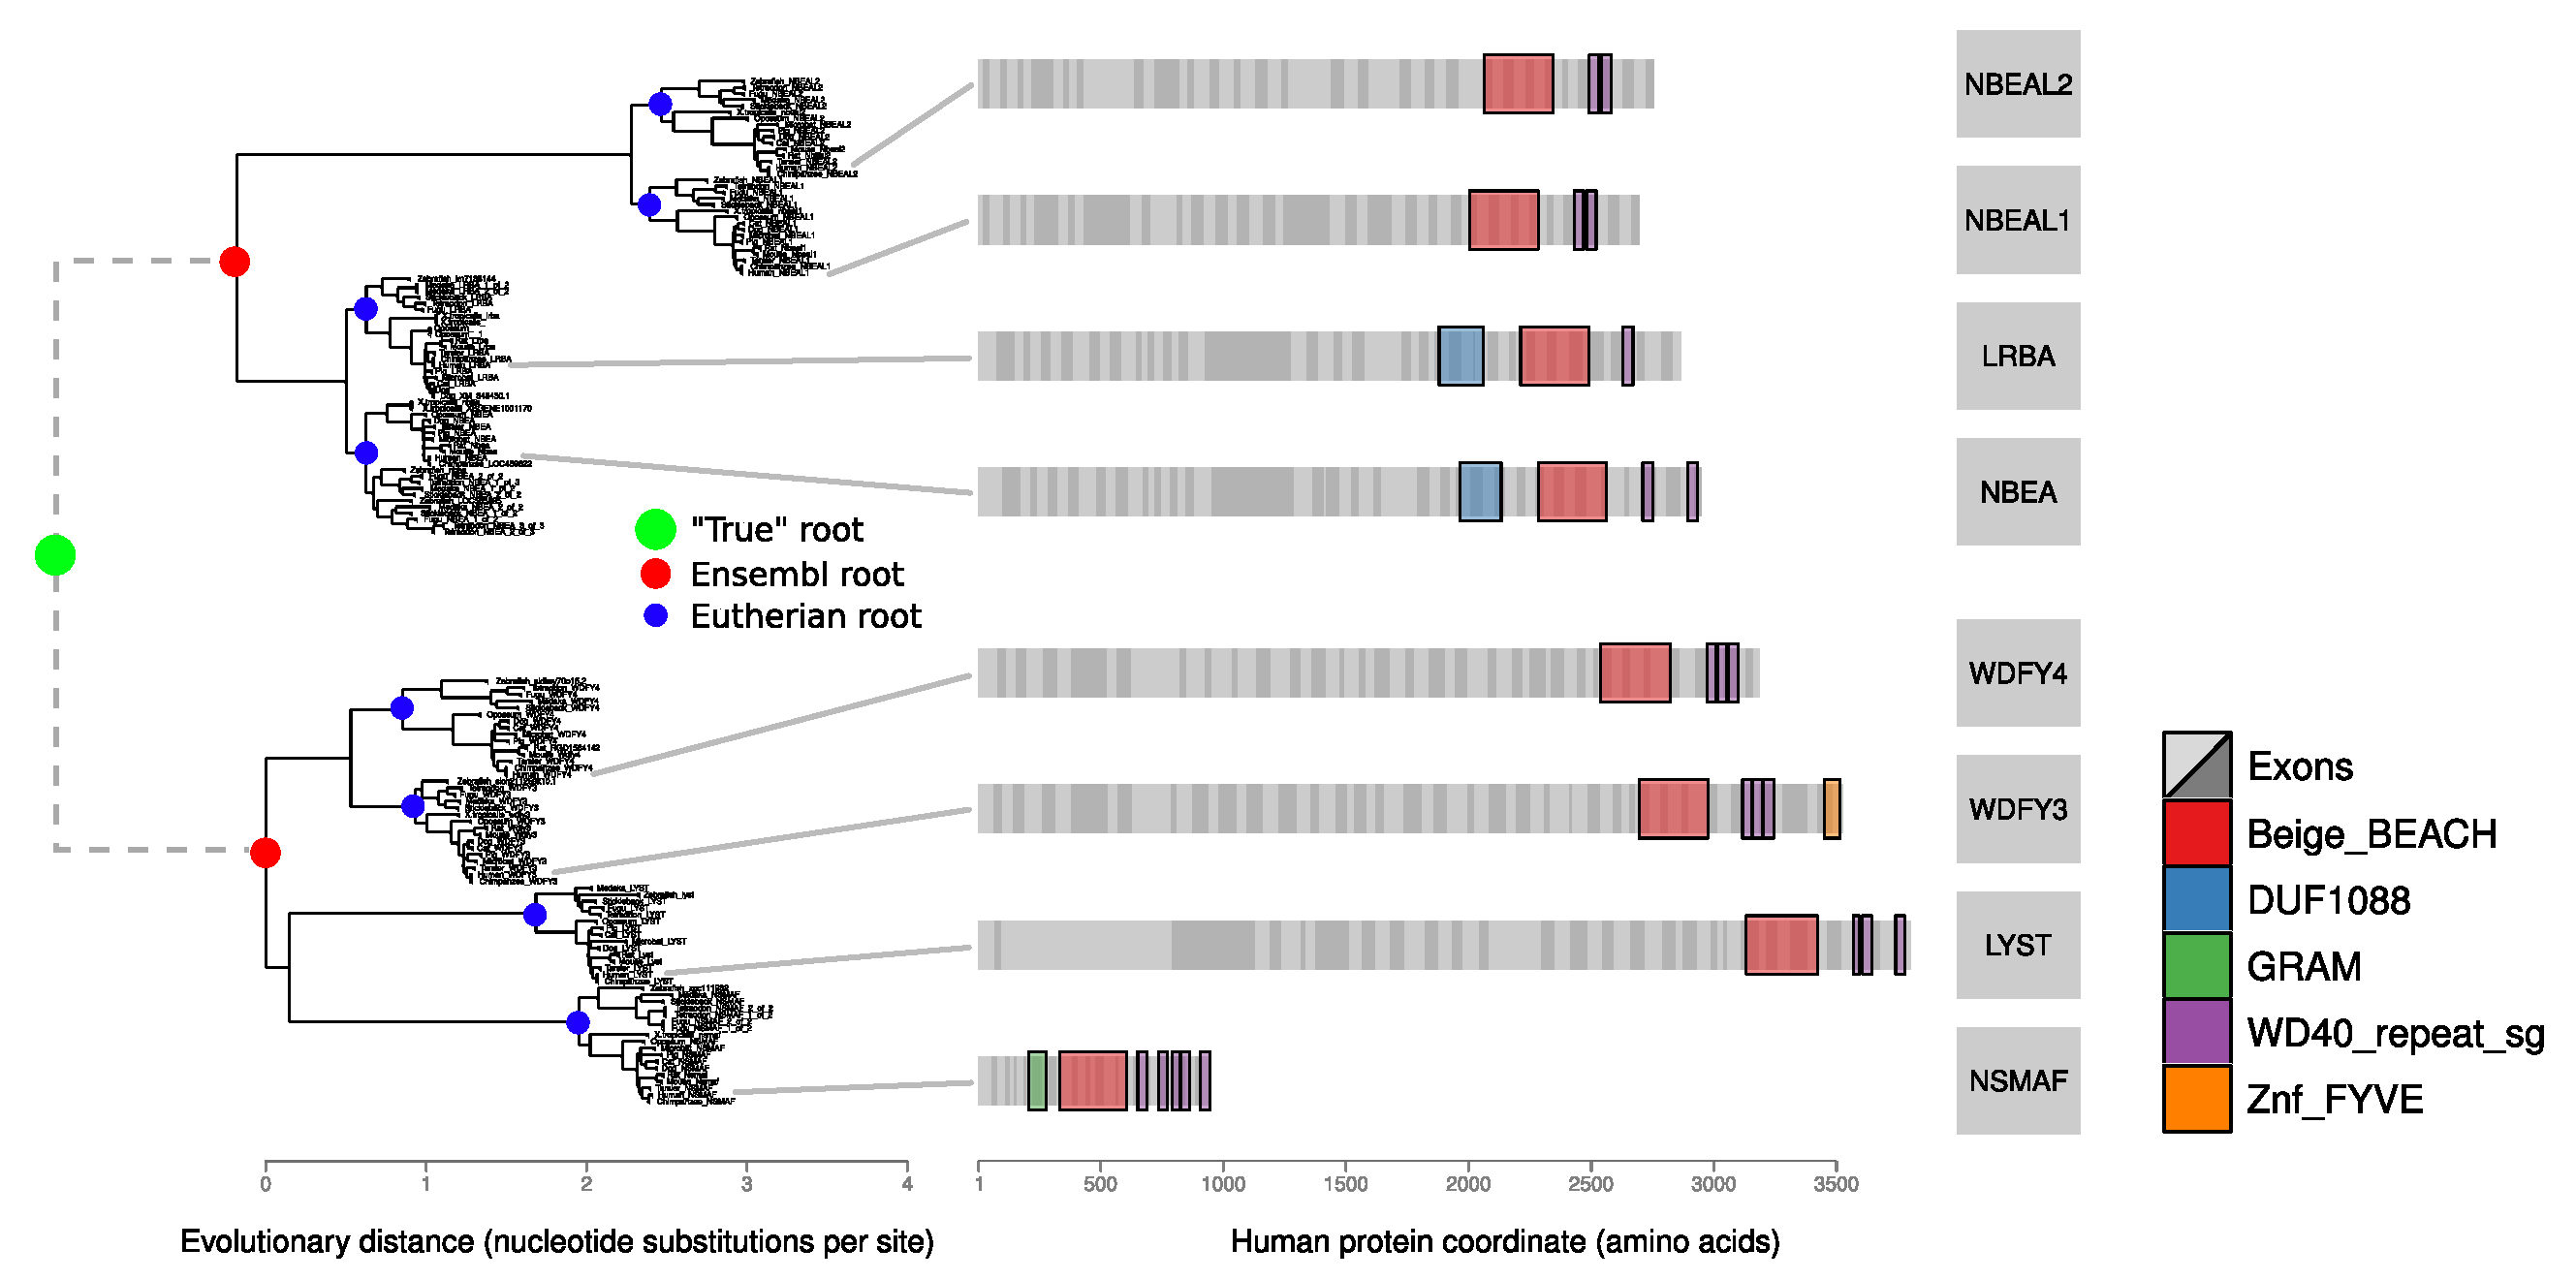
\includegraphics[scale=0.3]{Figs/nbeal2_full.pdf}
\caption{The evolutionary history of the human \gene{neurobeachin-like 2}
  gene (\gene{NBEAL2}) and its paralogs. Left, two phylogenetic trees from
  Ensembl Compara (release 60) are shown, summarizing the evolution of
  \gene{NBEAL2} and its three paralogs (top) and \gene{LYST}, a presumed distant
  paralog of \gene{NBEAL2}, and its three paralogs (bottom) in 15
  vertebrate species. The phylogeny shows that \gene{NBEAL2} is
  taxonomically conserved and distinct from its paralogs. Red dots
  highlight the root nodes of Ensembl gene trees, blue dots highlight
  the root nodes of Eutherian orthologous subtrees, and a dashed line
  with a green dot represents the putative paralogous relationship
  (with a hypothetical root) between the two Ensembl gene
  trees. Right, the exon and domain structure of each human gene is
  shown: exons are displayed alternating shades of gray, and Pfam
  domain annotations are colored according to their Pfam identifier.}
\label{nbeal2}
\end{figure}

Take for example the gene \gene{NBEAL2} and its human paralogs, whose gene
trees, exon structures and domain classifications were extracted from
Ensembl v62 and summarized in Figure \ref{nbeal2}. A recent medical
sequencing project identified \gene{NBEAL2}, a gene of previously unknown
function, as the putative causative gene for gray platelet syndrome, a
predominantly recessive platelet disorder resulting in moderate to
severe bleeding \citep{Albers2011}. It was important for the
purpose of this study to ensure that the \gene{NBEAL2} gene was both well-conserved
across mammals and distinct from its paralogs. The Compara pipeline
clustered \gene{NBEAL2} with three of its closest paralogs into one tree (and
similarly clustered four more distant \gene{NBEAL2} paralogs into a separate
tree), yielding two views which together showed both the full
taxonomic coverage of the \gene{NBEAL2} \subtr{} and the large amount of
separation between paralogs. Had each Eutherian ortholog been
displayed independently in Ensembl (using the blue ``Eutherian root'' nodes in
Figure \ref{nbeal2}), it would have been more difficult for a non-expert to make such
claims regarding the evolutionary history of \gene{NBEAL2} without further
analysis. Conversely, had the Compara pipeline been even more
inclusive in its clustering approach and identified the hypothetical deeper
root connecting these two sets of trees (represented by the green node
in Figure \ref{nbeal2}), the connection between these eight genes
would have been even more immediately apparent.

For the purposes of the current mammalian sitewise analysis, however,
it was important to isolate individual mammalian gene trees for
further processing and sitewise analysis. To this end, I designed a
simple scheme for splitting gene trees into non-overlapping subtrees
based on flexible taxonomic coverage criteria.

I hypothesized that a relatively simple set of rules based on
taxonomic coverage would be sufficient to identify most largely
orthologous mammalian subtrees. This hypothesis was based on two
well-established observations in mammalian genomes. First, the
existence of two rounds of whole-genome duplication preceding the
evolution of vertebrates \citep{Dehal2005} suggested that many of the
ancient duplication events contained within Ensembl gene trees
occurred before the divergence of \mmls, making it possible to cleanly
separate out taxonomically complete \mmln \subtr{}s in the majority of
cases. This would not be possible if duplication events were common
and spread evenly throughout the \mmln tree; if that were the case,
many duplication events would have occurred after the divergence of
some or all of the major \mmln groups, resulting in a larger
proportion of \mmln genes with ``internal'' duplications and, thus,
fewer singly orthologous trees with high taxonomic coverage. Second,
the overall low rate of gene duplication and loss in mammals
\citep{Demuth2006} (excluding, of course, the
aforementioned whole-genome duplication events) predicts that few
mammalian gene trees will be subject to one or more gene duplication
or loss events. In other words, most mammalian gene trees should
contain sequences from a majority of mammalian species, so the
effectiveness of using taxonomic coverage to identify mammalian
\subtr{}s should be largely unaffected by individual (i.e., post-2R)
gene duplication or loss events. The potential utility of taxonomic
coverage was further bolstered by the star-like shape of the mammalian
tree: star-like trees contain more branch length within terminal
lineages than ladder-like trees with an equivalent total branch
length, making it less likely that a gene duplication or loss event
(if such events occurred randomly throughout the mammalian tree) would
result in a significant disruption to the taxonomic coverage of the
gene tree.

The taxonomic-based tree splitting scheme works as follows. For every
internal node $N$ of each Compara gene tree, the \ac{tc} was calculated for several vertebrate clades. The \ac{tc} for node $N$
and clade $C$ is given by $TC(N,C) = species(N) / species(C) $, where
$species(N)$ is the number of unique species represented by the
sequences beneath node $N$ and $species(C)$ is the number of species
within the vertebrate clade $C$. The tree is traversed from root to
tip, and if a given set of \ac{tc} constraints (referred to as the subtree
constraints) are satisfied by both \subtr{}s below node $i$, then the
tree is split into two \subtr{}s at node $i$ (with the new trees
having root nodes placed at the two child nodes, $i_a$ and $i_b$). The
traversal continues recursively until every node is tested. If only
the original root node satisfies the subtree constraints, then the
entire Compara tree is included in the resulting tree set; if the
entire Compara tree fails to satisfy the subtree constraints, it is
excluded altogether.

I chose a variety of subtree constraints based on the structure of the
vertebrate phylogeny, all of which were run against the 18,613 gene
trees within the Compara database to generate several genome-wide sets
of subtrees. Table \ref{subtree_constraints} shows the details of the
various subtree constraints I used; the clade names (e.g.,
$TC(Primates)$) are used to refer to sets of species contained within
the Ensembl database, as defined by the NCBI taxonomy. The NCBI
taxonomy of species contained in Ensembl is shown in Figure
\ref{ncbi_tree}.

For the Ingroup and Outgroup categories of subtree constraints, a \ac{tc}
value of greater than 0.6 was required for a single taxonomic
clade. If the required \ac{tc} value for a clade were set to 1, then all
subtrees containing deletions in any species within the clade of
interest would be rejected. On the other hand, requiring a \ac{tc} value of
less than 0.5 would allow for a truly singly-orthologous tree to be
split into two \subtr{}s, with one tree having a \ac{tc} below 0.5, and the
other tree (containing the other half of the species) also having a \ac{tc}
below 0.5. Thus, 0.6 seemed to be a reasonable \ac{tc} requirement for
isolating \subtr{}s with reasonable taxonomic coverage while allowing
for some amount of gene deletion.

Two additional types of constraints were designed for use in the
MammalSubgroups and MammalSubgroupsPlusOutgoup methods. Inspired by
the alignment filtering method from Pollard et al. \citeyearpar{Pollard2010},
which required sequence data from all three major mammalian clades
(Primates, Glires, and Laurasiatheria) to be present for a column to
pass through the filter, the $TC_{all}$ constraint requires that the
\ac{tc} for all of the included clades is above a given threshold. To
complement the $TC_{all}$ constraint, the $TC_{any}$ constraint
requires that the \ac{tc} for any of the included clades is above a given
threshold. These more complicated methods were included in the
analysis in case the simpler \ac{tc} constraints within the Ingroup and
Outgroup categories did not perform satisfactorily.

The methods within the Orthologs category of subtree constraints were
implemented separately from the rest. Instead of splitting Compara
trees based on taxonomic criteria, the subtrees in the Orthologs
category were defined from the sets of genes annotated by Ensembl as
orthologs to each gene from a given source species. Thus, for each
gene from the source species, the Compara \subtr{} containing all of
the Ensembl-annoated orthologs was extracted and stored; this was
guaranteed to yield exactly one \subtr{} for every gene in the source
species. I chose to include human, mouse, zebrafish, and drosophila
were chosen as source species for testing. This approach differs from
the tree-splitting strategy in two ways: first, it makes use of the
orthology annotations resulting from Ensembl's orthology pipeline, and
second, it does not guarantee that each \subtr{} contains a completely
unique set of genes. For example, a gene which was recently duplicated
in humans would yield two \subtr{}s, one for each human paralog, with
identical sets of non-human genes in each tree. Although the
orthology-based method might be useful when an evolutionary study is
focused on a specific target or reference species, as is often done
with human and mouse due to their finished genome sequence and
high-quality annotation, I considered it to be less applicable to the
current study due to the potential for introducing reference
genome-specific biases, such as over-representation of genes with gene
family expansions in the reference species or non-representation of
genes which have been deleted in the reference species. Still, I
expected that the sets of \subtr{}s resulting from the Ensembl
ortholog annotations would serve as a useful reference with which to
compare the other \ac{tc}-based methods.

\begin{figure}
\centering
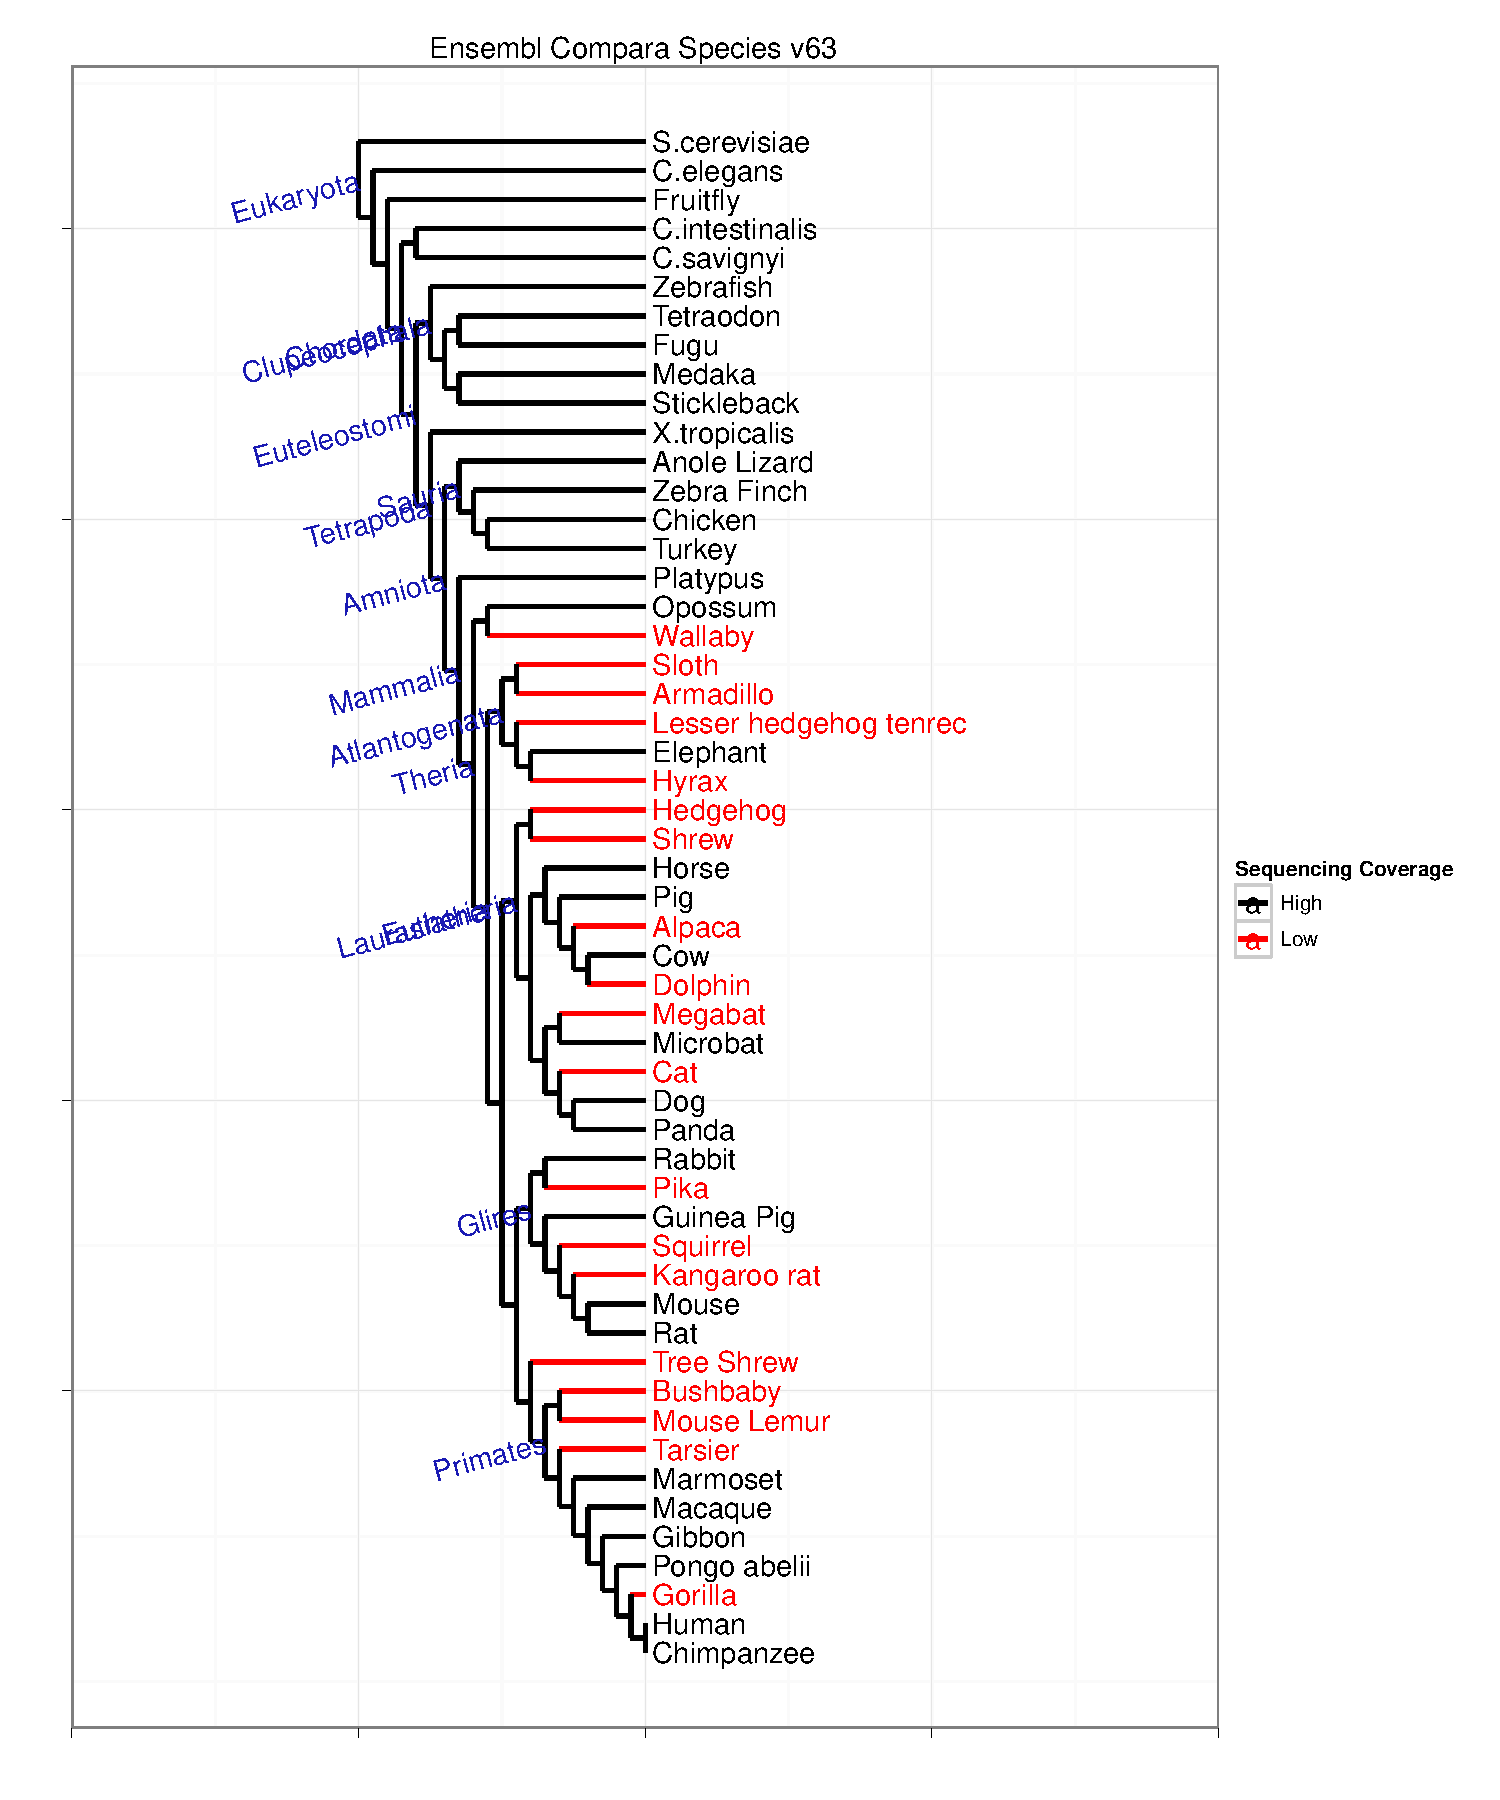
\includegraphics[scale=0.6]{Figs/compara_63_tree.pdf}
\caption{The NCBI taxonomy of species within the Ensembl Compara
  database. Note that branch lengths are not drawn to
  scale. Low-coverage genomes are labeled in red, high-coverage
  genomes are in black. Selected internal nodes, used are labeled in
  blue.}
\label{ncbi_tree}
\end{figure}


\begin{table} \footnotesize
\centering
\begin{tabular}{@{}lll@{}} \toprule
\multicolumn{2}{c}{Method} \\ \cmidrule(r){1-2}
   Category & Name & Constraints \\ \midrule
Ingroup & Primates & $TC(Primates) > 0.6$ \\
 &   Glires &  $TC(Glires) > 0.6$ \\
 &   Laurasiatheria & $TC(Laurasiatheria) > 0.6$ \\
 &   Sauria & $TC(Sauria) > 0.6$ \\
 &   Fish & $TC(Clupeocephala) > 0.6$ \\
Outgroup &  Eutheria & $TC(Eutheria) > 0.6$ \\
 &   Amniotes & $TC(Amniota) > 0.6$\\
 &   Vertebrates & $TC(Vertebrata) > 0.6$\\
 &   Fungi/Metazoa & $TC(Fungi/Metazoa) > 0.6$\\
Subgroups &  MammalSubgroups & $TC_{all}(Laur., Glires, Primates) > 0.1$\\
 &   \scriptsize{MammalSubgroupsPlusOutgroup} & $TC_{all}(Laur., Glires, Primates) > 0.1$ AND \\
 &    & $TC_{any}(Sauria, Clupeo., Ciona, Marsup.) > 0)$ \\
Orthologs & Human Orthologs & \\
 &   Mouse Orthologs &  \\
 &   Zebrafish Orthologs &  \\
 &   Drosophila Orthologs &  \\
Root Nodes & Ensembl Roots &  \\
\bottomrule
\end{tabular}
\caption{Subtree constraints used for identifying Eutherian
  orthologous subtrees. Ensembl gene trees were split into subtrees
  based on \acf{tc} requirements at internal
  nodes. Laur. - Laurasiatheria; Clupeo. - Clupeocephala; Marsup. -
  Marsupiala}
\label{subtree_constraints}
\end{table}

\section{Analysis of genome-wide sets of orthologous mammalian trees}

The \subtr splitting schemes described in the previous subsection were
applied to the 18,607 root gene trees from the Ensembl database. In
this and the next section I will describe the resulting sets of trees
and \subtr{}s, discuss what they reveal about the evolutionary history
of vertebrates and the feasibility of using taxonomic coverage to
isolate orthologous trees for sitewise analysis, and finally, explain
my reasoning for deciding to use the subtrees based on the Eutherian
taxonomic coverage for the subsequent sitewise analysis.

\subsection{The set of root Compara gene trees}

Table \ref{ensembl_root_table} presents a summary of the set of root
Compara gene trees and the subsets of trees with more or fewer than 15
sequences.

\begin{table} \footnotesize
\centering
\begin{tabular}{lrb{2cm}rrrrrrr}
\toprule
Tree & &  Med. Size &  & \multicolumn{3}{c}{Human Content} & Human & Med. & Med. \\ \cmidrule(r){5-7}
Set & Count  & (Min / Max) & N50 & 0 & 1 & 2+ & Total & MPL & Species \\ 
  \midrule
\input{Tables/ortholog_roots_summary.txt}
   \bottomrule
\end{tabular}
\caption{Summary of the set of Ensembl Compara root trees. The 'Human
  Content' columns represent the fraction of trees which contain the
  indicated number of human genes, and 'Human Total' is the total
  number of human genes contained within the tree set. 'Med. Species'
  is the median species count across all trees. Med. - median, MPL -
  mean path length }
\label{ensembl_root_table}
\end{table}

It is somewhat surprising that nearly half of all Compara gene trees
contain few sequences: 9,378 out of 18,607 root trees constitute fewer
than 15 sequences. Given the protein-based clustering performed by the
Compara pipeline, one might expect many of these small trees to
represent portions of larger fast-evolving gene trees whose high
sequence divergences made the BLAST search step inaccurate or caused
clustering via the \hclust algorithm to be ineffective. Alternatively,
these small clusters might have resulted from exceptional
lineage-specific gene duplications or pseudogenes mis-annotated as
genes, creating tight clusters of very closely-related transcripts
that were identified by \hclust as independent gene trees. Some
evidence for the latter scenario comes from the median species counts
and mean path lengths of the smaller versus larger trees. The subset
of small root trees has a median species count of 2 compared to 47 for
the large subset, indicating that the smaller trees encompass
sequences from a very small taxonomic range. Furthermore, the median
MPL for small trees is 0.04 compared to 1.04 for the large subset,
revealing a much smaller level of sequence divergence within each
tree. Together, these summary statistics indicate that the smallest
trees in the Compara database consist of highly species-specific,
closely-related proteins that are likely artifactual gene
annotations.

Despite the existence of many small trees in the Compara database,
they comprise only a small fraction of all protein-coding
sequences. Only 4\% of the human gene set---which we expect to be
well-annotated and to contain few false positive genes due to the high
level of manual curation and the large amount of continued
scrutiny---is contained within the subset of small trees. This
indicates that whatever process is causing the Compara pipeline to
yield such a high number of small gene trees has not had too much of
an impact on the placement of the most confident set of protein-coding
genes within the database of root gene trees.

\begin{figure}
\centering
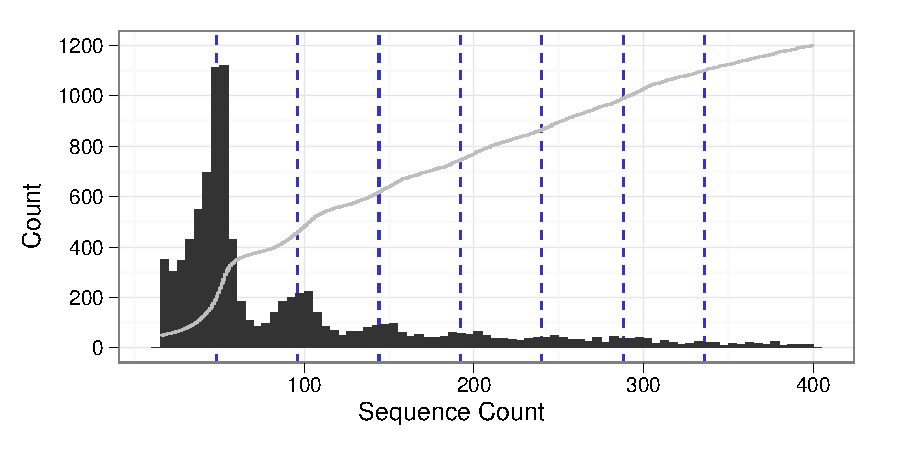
\includegraphics[scale=0.9]{Figs/ensembl_roots_hist.pdf}
\caption{Sequence counts for the set of root Compara trees. Black bars
  show a histogram of sequence counts in bins of width 5, and the gray
  line shows the cumulative fraction of sequences contained within
  trees of that size or smaller. For clarity, 9,378 trees with 15 or
  fewer sequences are not shown. Dashed blue lines are drawn at
  integral multiples of 48, the number of vertebrate species within
  Ensembl.}
\label{ensembl_roots_hist}
\end{figure}

A closer examination of the distribution of tree sizes in the set of
root Compara trees presents a clear view of the over-clustering of
mammalian orthologous trees. The black bars in Figure
\ref{ensembl_roots_hist} show the distribution of sequence counts for
all trees with more than 15 sequences, with vertical dashed lines
overlaid at multiples of 48 (the number of vertebrate species in
Ensembl release 63). The highest peak
of the histogram is at or slightly above 48 sequences, with the tree
counts quickly diminishing at larger sizes. Weaker, but still
discernable, peaks appear at larger tree sizes, with the location of
these echo-like peaks corresponding closely to the second, third and
fourth multiples of 48. The pattern of recurring peaks becomes
indistinguishable at sizes above 200, but there is still a long tail
of large trees extending out to a maximum size of 400
sequences. Overall, the distribution of tree sizes provides good
support for the situation described above, with the Compara pipeline
often clustering together two or more largely-orthologous gene trees
sharing ancient homology.

It is also interesting to characterize the set of Ensembl trees by the
proportion of all sequences which are covered by trees of a given size
or smaller. This value is plotted in Figure \ref{ensembl_roots_hist}
as a gray line. First, one can see that trees with fewer than 15
sequences (which were excluded from the plot but inlcuded in the
calculation of the cumulative fraction of sequences) represent a
trifling fraction of the sequences within Compara; this is similar,
but not identical, to the above-mentioned calculation that 4\% of
human genes are contained within these smaller trees. Second, the
steady slope of the cumulative curve contrasts with the declining
height of the histogram. This results from the increasing number of
sequences encompassed by each of the larger trees: although there are
relatively few trees with more than 300 sequences, together they
contain around 10\% of all protein-coding genes in Ensembl. Two points
along this cumulative plot are of particular interest. First, one can
identify the fraction of vertebrate proteins which exist as
identifiable paralogs. Looking at the value along the x-axis where the
largest bump in the histogram ends, at around 75 sequences, one can
see that in total around 30\% of proteins are covered by trees of 75
sequences or fewer. Since the pattern of bumps in the histogram
correlate well with the number of Ensembl vertebrate species, it would
be reasonable to state that 70\% of vertebrate proteins are contained
within large gene trees containing sequence-based evidence of ancient
paralogy. Second, a look-up in the reverse direction can identify the
tree size at which 50\% of sequences are clustered. This value
represents the size of tree that an ``average'' protein might be
clustered in, and in some ways is a more accurate characterization of
the set of gene trees than the median tree size. A similar calculation
is often performed to characterize the size distribution of contigs
(contiguous sequence blocks) within a genome assembly. This statistic,
referred to as the N50 length, is the contig length for which 50\% of
bases are contained in contigs of that size or larger
\citep{Miller2010}. For the Ensembl root trees, the N50 tree size is 139,
slightly less than three times the number of vertebrate species. The
N50 tree size is shown for the root trees in Table
\ref{ensembl_roots_hist} and in the table for taxonomically-defined
tree sets below.

Another way to characterize the distribution of gene trees is across
the taxonomic space. A question of particular interest to the
identification and analysis of mammalian orthologs is whether levels
of gene presence and absence are consistent across different species
and different levels of assembly quality. To investigate this question
in the context of the root Ensembl trees, data were collected by
counting the number of sequences from each species contained within
each gene tree. Results were tabulated for each species and are
presented in Figure \ref{ortholog_root_dups}, showing the number of
trees containing 0, 1, 2, or more than 3 genes from each of the 53
species in Ensembl. Comparing the range of values in the panels for
each copy count (labeled 0, 1, 2 and 3+), one finds that most trees
(8,000-11,000 within vertebrates) contain zero copies from a given
species, fewer trees contain one copy (4,000-6,000) and several
thousand contain two, three or more copies (ca. 1,000-1,500 for 2
copies and 1,500-2,000 for 3+). The plethora of trees with zero copies
from a given species is again a result of the existance of many small,
species-specific trees within the root Ensembl set. Similarly, the
high number of trees with many copies from each species reflects the
clustering of multiple orthologous sub-trees together.

A comparison of values across the range of species in Figure
\ref{ortholog_root_dups} reveals that the zero-copy count tends to
increase along with evolutionary distance from human, while the 1, 2
and 3+ copy counts tend to decrease as the distance from human
increases. Both trends are most striking at the distant end of the
tree where the five non-vertebrate species begin. For the increase in
zero-copy trees and the decrease in single-copy trees, the strength of
the trend at the highest level of divergence can be partly explained
by the very long branch lengths connecting those species to each other
and to the more well-represented vertebrate clade: the distance-based
clustering algorithm might reasonably be expected to produce more
false negatives in longer branches for a number of reasons including
the behavior of the \hclust algorithm, inaccurate BLAST E-values at
larger distances, and heterogeneity in evolutionary rates across
lineages \citep{Whelan2008}. However, the dearth of 2 and 3+ copy counts in
non-vertebrates is most likely a signal resulting from the 2R event at
the basal vertebrate lineage, with the non-vertebrate species strongly
depleted of multi-copy duplicates compared to their vertebrate
relatives.

It is slightly concerning that human and its close primate relatives
contain fewer zero-copy genes and more one-copy and two-copy genes
than any other group of vertebrates in the set of Ensembl trees. There
is no \emph{ab initio} biological reason to expect this to be the
case, and I suspect that the existence of such a pattern, which is
fairly small in effect, is due to the widespread reliance on human
annotation and protein experimental data in the annotation of
non-human genomes. There is one region where this trend does not
appear to be the case: in the 3+ copy count for the fish species,
which is instead a result of gene duplicates retained after the third
round of genome duplication which occurred in the teleost ancestor
\citep{Jaillon2004}. The signal resulting from the teleost genome duplication
event is clearer in the sets of taxonomically-defined \subtr{}s, so I
will defer its discussion to the next subsection where those sets of trees are described.

Finally, the differences in copy counts between species with low- and
high-coverage genome sequences show the tendency of low-coverage
genome sequences to yield false negatives in the gene annotation, as
low-coverage species contain more zero-copy, roughly the same number
of one-copy, and noticeably fewer multi-copy genes than high-coverage
species. These clear effects of low sequencing coverage show that gene
absence in low-coverage genomes should not be taken as evidence for
actual gene loss and that gene duplications are systematically
underrepresented in low-coverage genomes. The former point was
emphasized in a recent critical analysis of the effect of low-coverage
genomes on gene duplication inference \citep{Milinkovitch2010}, but
the latter point was largely ignored. Again, this signal is also
stronger in the more stringent set of \mmln orthologous \subtr{}s and
will be revisited in the next subsection.

The preceding analysis of the set of root Ensembl trees, in which I
characterised the distribution of trees with respect to size
(i.e. sequence count) and across the taxonomic space, showed that
despite the over-representation of small, species-specific trees, most
sequences are contained in trees with biologically plausible sizes
given the history of vertebrate genome duplications. The tree-based
equivalent of the N50 statistic was developed for summarizing the
distribution of differently-sized trees, and two main views of this
distribution were introduced (in Figures \ref{ortholog_root_dups} and
\ref{ensembl_roots_hist}), providing evidence for the clustering of
paralogous mammalian sub-trees and for species-based and genome
coverage-based trends in the breakdown of gene copy counts within
these trees.

\begin{landscape}
\begin{figure}
\centering
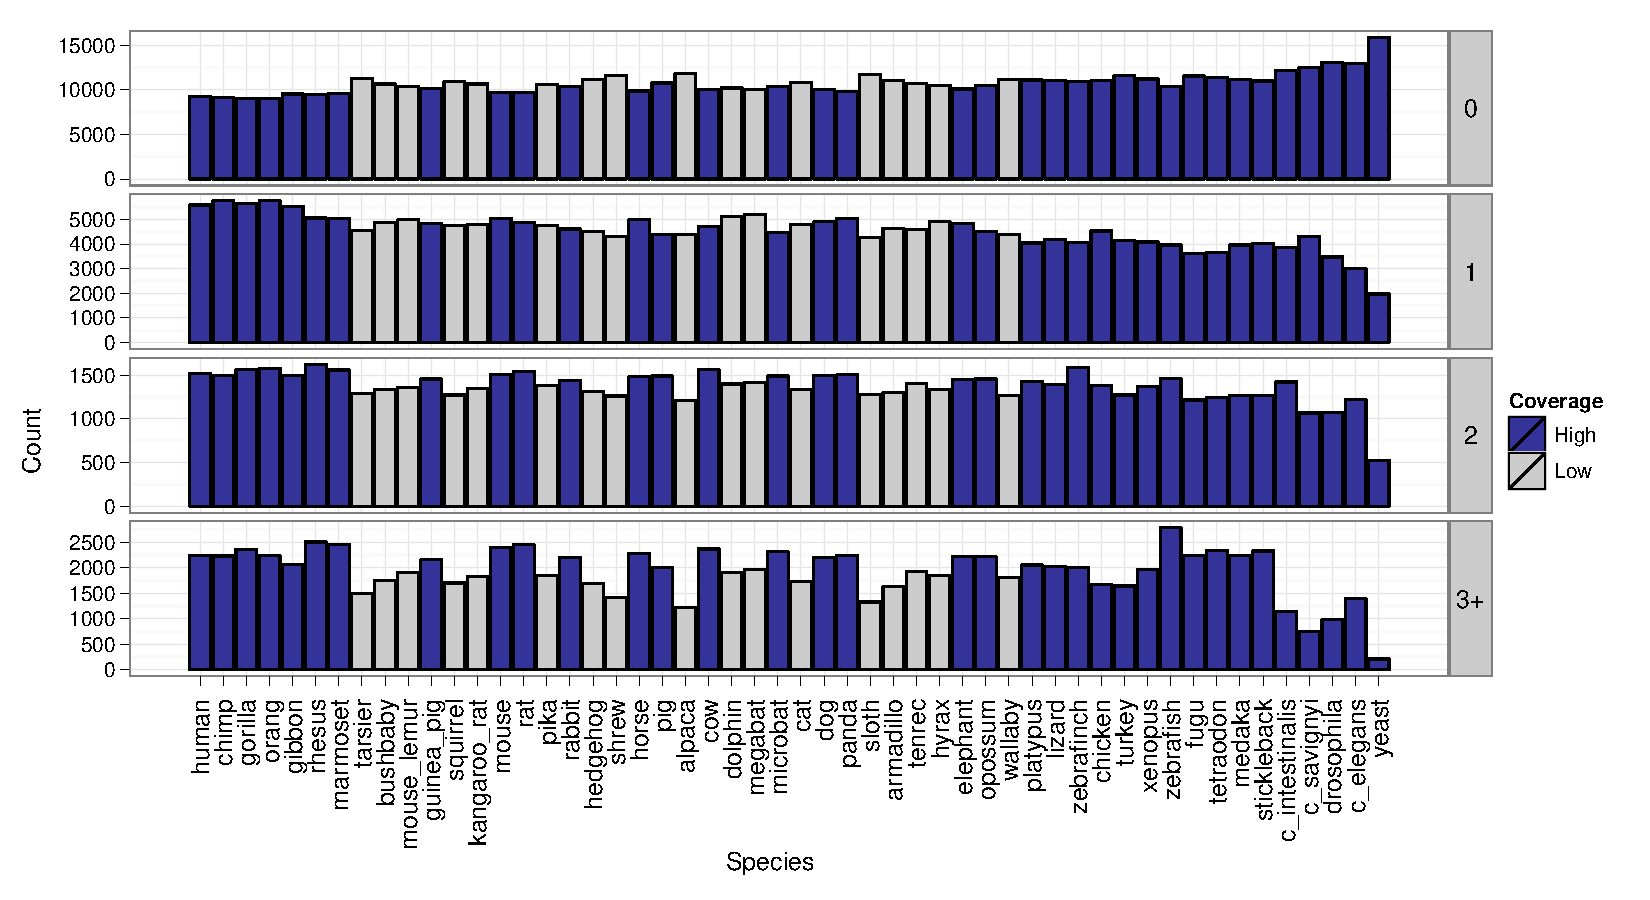
\includegraphics[scale=0.9]{Figs/ortholog_root_dups.pdf}
\caption{Taxonomic distribution of gene copy counts for the root
  Ensembl trees. The number of trees containing 0, 1, 2 or more than 3
  sequences from each species is shown. Bars are colored blue and gray
  for species with high- and low-coverage genomes, respectively. Note
  that the y-axis scale is not the same for each panel.}
\label{ortholog_root_dups}
\end{figure}
\end{landscape}

\subsection{Sets of \subtr{}s defined by taxonomic coverage and orthology annotation}

The sets of trees resulting from applying the various \subtr
extraction methods to the root Ensembl gene trees are summarised in
Table \ref{ensembl_subtree_table}, with the original Ensembl trees
included at the bottom for comparison.

The Ensembl Roots and Drosophila Orthologs sets are two clear
outliers, with much higher N50 values than any other set (139 and 125
vs. the next highest value of 56) and more trees with multiple human
copies (0.20 and 0.43 vs. the next highest value of 0.14). In fact,
the major differences between these sets are all attributable to the
excess of small species-limited trees in the Ensembl Roots group: the
Drosophila Orthologs set contains fewer trees than the Ensembl Roots
(9,210 vs. 18,607) and a larger average tree size (60 vs. 15), closely
resembling the set of Ensembl Roots with small trees removed as
summarised in the third row of Table \ref{ensembl_root_table}.

Within the Ingroup category of methods, the methods based on
mammalian \ac{tc} values (Primates, Glires and Laurasiatheria) produced
largely similar sets of trees, with the Primate set containing around
2,000 more trees and covering around 1,000 more human genes than the
other two sets. A reason for the higher number and human coverage of
Primate trees is not immediately apparent, although it may
speculatively be due to an excess of primate-specific gene trees that
are not captured by non-primate \ac{tc}-based criteria. Further
investigation of the trees unique to this set might reveal the root
cause of this slight discrepancy.

The Sauria and Fish tree sets stood in strong contrast to the
mammal-based methods from the Ingroup category. The Sauria clade is
represented by only four Ensembl species and diverged from the
mammalian ancestor at an early point in the evolution of amniotes. The
moderately lower number of trees (13,046 vs. 15,764 for
Laurasiatheria) and the increased proportion of trees containing
multiple human genes (0.14 vs. 0.09 for Laurasiatheria) are presumably
consequences of the lower clade size, which could affect the \ac{tc}
calculation, and the long branch separating Sauria from the other
vertebrate clades. The fish-based subtree constraint produced a
strikingly different set of trees resulting from the impact of the
teleost-specific whole genome duplication on the structure of fish
gene trees. Although the Fish tree set contains a N50 value of 49
which is no different from the N50 of the other Ingroup sets, Table
\ref{ensembl_subtree_table} highlights three major differences in the
Fish set: it contains many more trees, a higher proportion of trees
with zero human copies, and a lower total human gene count than the
other Ingroup sets.

The reason for the drastically different Fish tree set is that the
tree splitting procedure identifies largest non-overlapping \subtr{}s
that satisfy the given \ac{tc} criteria. Genes that were duplicated in the
teleost lineage and retained in duplicate form (as opposed to one or
both copies being lost in either of the descendant duplicate
chromosomes) would result in a gene tree with two teleost-specific
\subtr{}s, each containing a high \ac{tc} value for the Clupeocephala
clade. In this case, the splitting procedure would result in two small
Fish subtrees, ``missing'' the single subtree of mammalain orthologs
because two non-overlapping trees already exceeded the \ac{tc} threshold of
0.6. If, however, one of the duplicate gene copies were lost, then the
tree would resemble a typical singly-orthologous vertebrate gene tree,
and the splitting procedure would select a \subtr encompassing the
entire vertebrate clade. It follows that the presence of small,
teleost-specific gene trees in the Fish set is a signal of retained
duplicate copies, and the size distribution of trees from the Fish
set, shown in Figure \ref{ensembl_fish_hist}, shows that several
thousand trees fit the expected model. If we assume that all trees
from the Fish subset which contain zero human copies, span 5 or fewer
species, and contain 40 or fewer sequences are likely retained
duplicate genes, a total of 6,980 retained duplicates are identified,
yielding a retention rate of 17.5\%, which is very much in line with a
previously published estimate of 15\% based on a comparison of
tetraodon, fugu and zebrafish genes \citep{Brunet2006}.

\begin{figure}
\centering
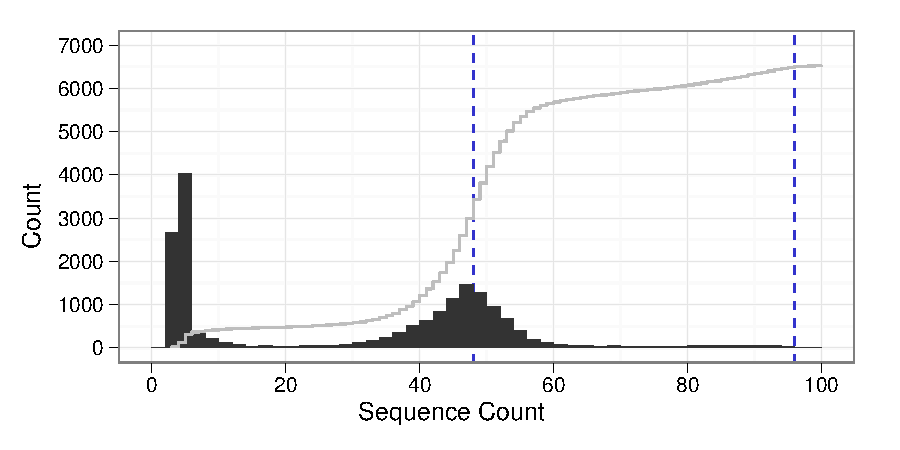
\includegraphics[scale=0.9]{Figs/ensembl_fish_hist.pdf}
\caption{Sequence counts for the set of \subtr{}s identified using the
  Fish clade taxonomic coverage constraint, showing an excess of small
 \subtr{}s resulting from the teleost genome duplication. Black bars show a
  histogram of sequence counts in bins of width 2, a gray line shows
  the cumulative fraction of sequences contained within trees of that
  size or smaller, and dashed blue lines are drawn at integral
  multiples of 48, the number of vertebrate species within
  Ensembl. The 255 trees with more than 100 sequences are not shown.}
\label{ensembl_fish_hist}
\end{figure}

The sets of \subtr{}s resulting from the Outgroup methods were of
special interest, as the clades used to define these \ac{tc} constraints
contained all or nearly all of the mammalian species whose orthologous
genes I wished to study. The resulting sets of \subtr{}s showed little
variation, owing perhaps to the large sizes of the clades and their
similar composition. Each set contained between 15 to 17 thousand
trees, N50 values of around 49, and greater than 90\% of trees
containing exactly one human sequence. These measures provided good
evidence that the tree-splitting method was effectively isolating
singly orthologous mammalian trees.  Some slight trends were apparent,
however, with the tree count decreasing, the proportion of trees with
human duplications increasing, and the overall human gene coverage
decreasing as the clade size used for the \ac{tc} calculation
increased. These trends could understandably be the result of the
minimum required tree size increasing along with the clade size,
ranging from 21 for Eutheria to 32 for Fungi/Metazoa.

The Subgroups methods did not appear to produce \subtr{}s of any
higher quality or more biological interest than the Outgroup
methods. The MammalsSubgroups set was more numerous than the Outgoups
sets, but the N50 was slightly lower (46 vs. 49) and the proportion of
zero-humany trees was higher (0.18 vs. 0.01), suggesting that the
additional trees were spurious results containing fragmented species
coverage. The addition of an outgroup requirement to the
MammalSubgroupsPlusOutgroup method produced a tree set more closely
resembling the Outgroup methods, but the human gene coverage was
lower than that for any Outgroup method despite the overall higher
tree count.

Finally, the ortholog annotation-derived \subtr{}s provided for an
interesting comparison between three different ortholog sources and
between the overlapping and non-overlapping sets of \subtr{}s. As I
mentioned at the beginning of this section, the \species{Drosophila}
ortholog set was highly contrasted with the vertebrate sets due to the
two rounds of whole genome duplication. There was minimal variation
among the other ortholog sets, although it is interesting to note that
Ensembl contained 21,873 mouse protein-coding genes while human
contained only 19,991. Zebrafish, on the other hand, contained 24,540
genes, in line with the 17.5\% rate of duplicate gene retension I
estimated earlier. Overall, 76\% and 81\% of mouse and zebrafish genes
have an apparent one-to-one ortholog in human, which is slightly lower
than the 92\% of Eutheria \subtr{}s containing one human sequence.

\begin{landscape}
% latex table generated in R 2.13.0 by xtable 1.5-6 package
% Thu Sep 15 11:19:59 2011
\begin{table}
\centering
\begin{tabular}{llrb{2.5cm}rrrrrrr}
\toprule
\multicolumn{2}{c}{Method} & &  Med. Size &  & \multicolumn{3}{c}{Human Content} & Human & Med. & Med. \\ \cmidrule(r){6-8} \cmidrule(r){1-2}
Category & Name & Count  & (Min / Max) & N50 & 0 & 1 & 2+ & Total & MPL & Species \\ 
  \midrule
\input{Tables/ortholog_summary.txt}
\bottomrule
\end{tabular}
\caption{Summary of Ensembl \subtr{}s identified using taxonomic
  criteria or Ensembl ortholog annotations. The set of Ensembl root
  trees (``Ensembl Roots'') from Table \ref{ensembl_root_table} is
  included for comparison. Cells in numeric columns are shaded
  according to their value relative to other rows, with low values in
  white and high values in blue. The 'Human Content' columns represent
  the fraction of trees which contain the indicated number of human
  genes. 'Med. Species' is the median species count across all
  trees. Med. -- median, MPL -- mean path length}
\label{ensembl_subtree_table}
\end{table}
\end{landscape}

Figure \ref{ortholog_stacked_bar} shows the taxonomic distribution of
gene copy counts for the trees resulting from each of the \subtr
methods tested. By way of reference, the values shown in the separate
panels of Figure \ref{ortholog_root_dups} appear in Figure
\ref{ortholog_stacked_bar} as different-colored bars in the bottom
panel. Although the various characteristics of each of the \subtr
methods have already been discussed at length, the taxonomic view
reveals some salient features of the patterns of gene deletion and
duplication within the tree sets and shows the pervasive impact of
genome-wide duplications on the evolution of vertebrate genes. The
large fraction of species with multiple copies in Drosophila Orthologs
\subtr{}s is a result of the two rounds of vertebrate genome
evolution, while the elevated fraction of multi-copy fish trees in the
Outgroup \subtr{}s shows the impact of the teleost-specific
duplication event.

Furthermore, the relative prevalence of zero-copy and multi-copy trees
can provide some indication of whether gene deletion or gene
duplication is a more common process in vertebrate genomes. Focusing
on the four Outgroup \subtr methods, the observation of a greater
number of multi-copy trees than zero-copy genes, valid across all four
\subtr methods and throughout all mammalian species except platypus,
can be interpreted as tentative evidence for a greater number of gene
duplications than gene deletions in the evolution of mammalian
genomes. This pattern does not hold for vertebrates more distantly
related to human, however: vertebrates beyond opossum show a distinct
and consistent increase in zero-copy trees, and birds appear to
exhibit a slight clade-specific drop in the proportion of multi-copy
trees. Of course, both of these trends could be methodological
artifacts related to the \hclust algorithm or to the methods used to
assemble and annotate more distantly-related genomes.

The distributions in Figure \ref{ortholog_stacked_bar} also reveal the
pig to harbor a very high number of apparent gene deletions, unmatched
by other mammalian species and nearing the proportion of zero-copy
trees seen in platypus and more distant vertebrates. Given the
consistently low proportion of zero-copy trees for other
closely-related species, I would expect this number to change once a
finished-quality pig genome sequence is included in the Ensembl
pipeline \citep{Archibald2010}.

\begin{figure}
\centering
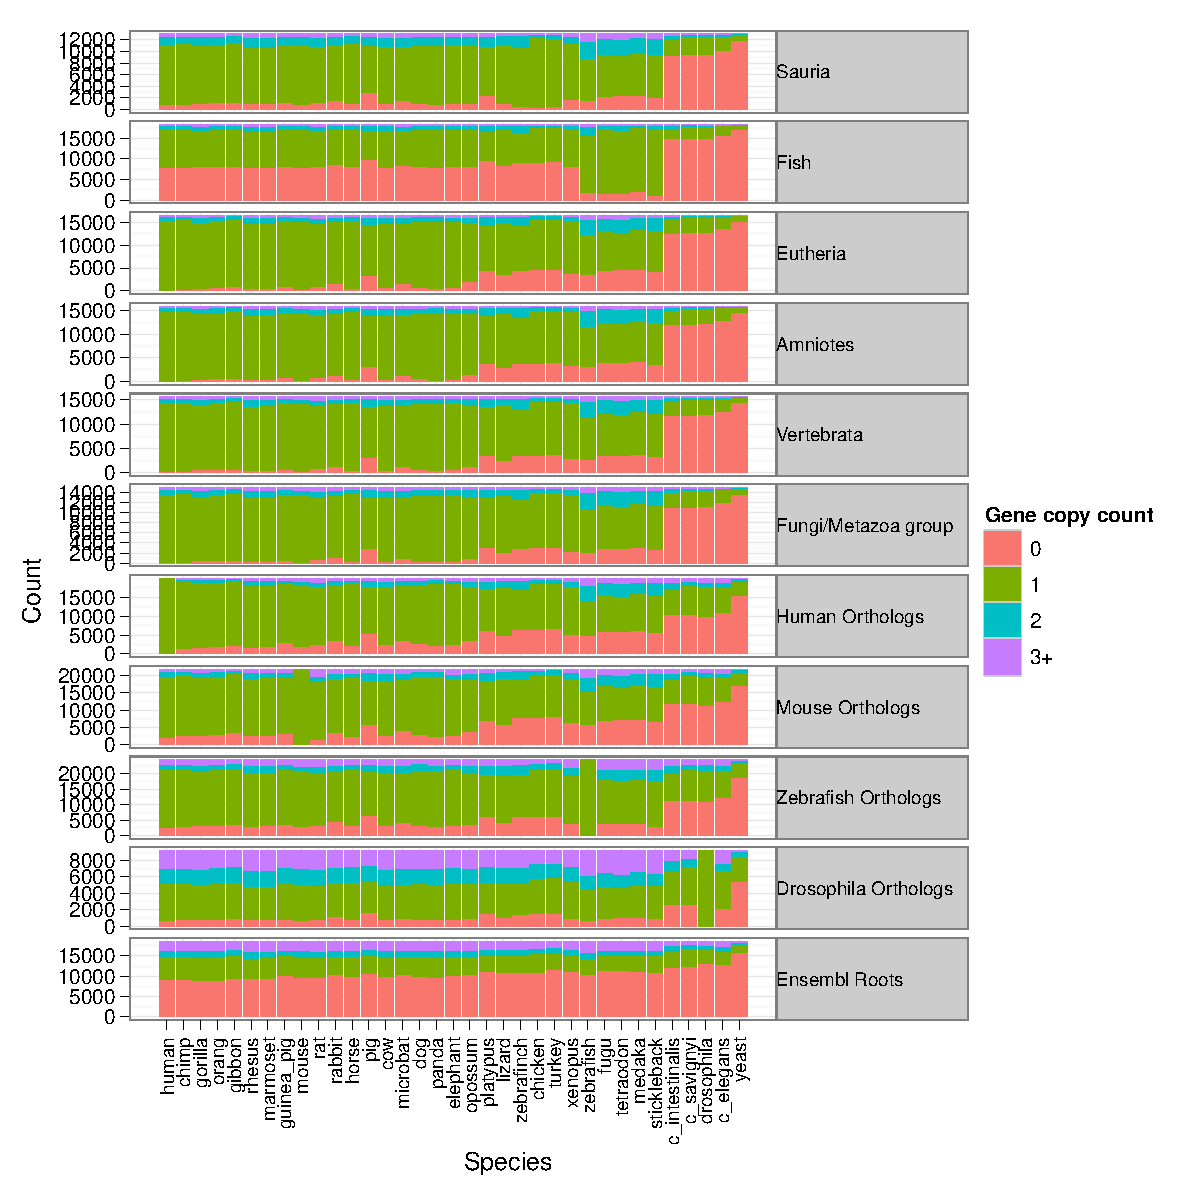
\includegraphics[scale=0.8]{Figs/ortholog_stacked_bar.pdf}
\caption{Taxonomic distribution of gene copy counts for different
  \subtr methods. The numbers of trees containing 0 (red), 1 (green),
  2 (blue) or more than 3 (purple) sequences from each species are
  shown as stacked colored bars. The Ingroup and Subgroups methods
  were omitted for clarity, as were species with low-coverage
  genomes. Note that the y-axis scale is not the same for each panel.}
\label{ortholog_stacked_bar}
\end{figure}

In the end, the set of Eutheria \subtr{}s was chosen as the final set
for use in the downstream evolutionary analysis, due to the slightly
larger number of trees and better coverage of human genes in the
Eutheria set compared to the other Outgroup methods. The distribution
of tree sizes for the Eutheria set of \subtr{}s is shown in Figure
\ref{ensembl_euth_hist} and the full taxonomic distribution of copy
counts is included in Figure \ref{ortholog_euth_dups}.

\begin{landscape}
\begin{figure}
\centering
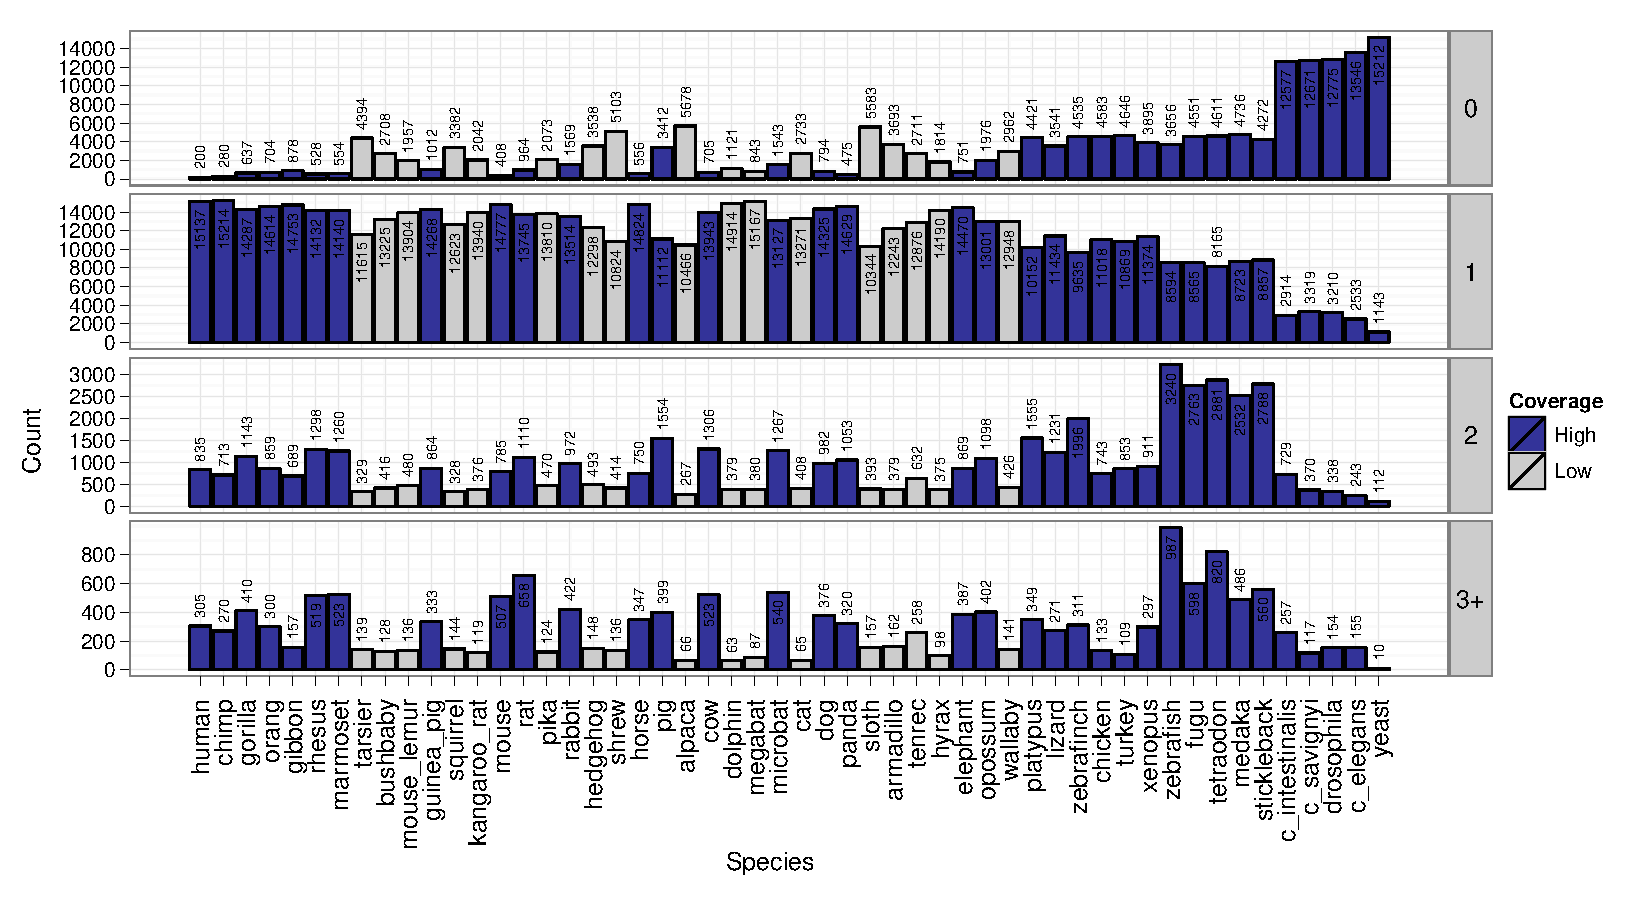
\includegraphics[scale=0.9]{Figs/ortholog_euth_dups.pdf}
\caption{Taxonomic distribution of gene copy counts for the Eutheria
  \subtr{}s defined by \ac{tc}. The number of trees containing 0, 1, 2 or more than 3
  sequences from each species is shown. Bars are colored blue and gray
  for species with high- and low-coverage genomes, respectively. Note
  that the y-axis scale is not the same for each panel.}
\label{ortholog_euth_dups}
\end{figure}
\end{landscape}

\begin{figure}
\centering
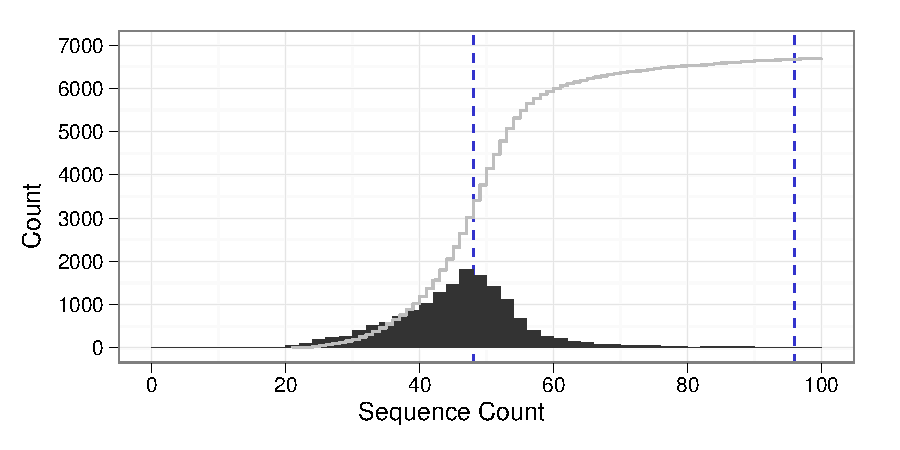
\includegraphics[scale=0.9]{Figs/ensembl_euth_hist.pdf}
\caption{Sequence counts for the set of \subtr{}s identified using the
  Eutheria clade taxonomic coverage constraint. Black bars show a
  histogram of sequence counts in bins of width 2, a gray line shows
  the cumulative fraction of sequences contained within trees of that
  size or smaller, and dashed blue lines are drawn at integral
  multiples of 48, the number of vertebrate species within
  Ensembl. The 230 trees with more than 100 sequences are not shown.}
\label{ensembl_euth_hist}
\end{figure}

\section{Conclusions}

\draft{Restate the goals: figure out which \ac{tc} criteria could be used to isolate largely-orthologous mammalian gene trees}
